\documentclass[final]{beamer}
\usepackage[orientation=landscape, size=custom, width=100cm, height=70cm, scale=1.5]{beamerposter}

\usepackage[swedish]{babel}
\usepackage[T1]{fontenc}
\usepackage[utf8]{inputenc}

\usepackage{lmodern}
\usepackage{hyphenat}
\usepackage{microtype}
\usepackage{parskip}
\usepackage{float}
\usepackage{graphicx}
\usepackage{booktabs}

\usebackgroundtemplate{
\includegraphics[width=\paperwidth]{figures/header.pdf}}

% https://www.komm.umu.se/grafisk-profil/
\definecolor{umublue}{RGB}{0,61,165}
\definecolor{umulightblue}{RGB}{0,160,230}
\definecolor{umugreen}{RGB}{80,190,31}

\setbeamercolor{titlelike}{fg=white}
\setbeamercolor{author}{fg=white}
\setbeamercolor{institute}{fg=white}
\setbeamercolor{block title}{fg=umublue,bg=white}
\setbeamercolor{block body}{fg=black,bg=white}
\setbeamercolor{block alerted title}{fg=white,bg=umublue}
\setbeamercolor{block alerted body}{fg=black,bg=dblue!10}

\newlength{\onecolwid}
\setlength{\onecolwid}{0.2\textwidth} % Width of one column

\title{Vattenrening med robotflotte}
\author{Anton Eriksson, Emelie Nordlinder, Jenny Bergman,
  Jesper Vesterberg, Joel Vedin, Johan Olofsson, Rasmus Nyman}
\institute{Design-Build-Test Grupp 5, Umeå Universitet}

\usepackage{atbegshi}% http://ctan.org/pkg/atbegshi
\AtBeginDocument{\AtBeginShipoutNext{\AtBeginShipoutDiscard}}

\begin{document}

\addtobeamertemplate{block end}{}{\vspace*{2ex}} % White space under blocks
\addtobeamertemplate{block alerted end}{}{\vspace*{2ex}} % White space under highlighted (alert) blocks

\setlength{\belowcaptionskip}{2ex} % White space under figures
\setlength\belowdisplayshortskip{2ex} % White space under equations

\begin{frame}[t]

  \begin{columns}[c]
    \begin{column}{\textwidth}
      \centering
      \vskip 1cm
      \usebeamercolor{title in headline}{\color{white}\Huge{\textbf{\inserttitle}}\\[0.5ex]}
      \usebeamercolor{author in headline}{\color{white}\insertauthor\\[0.8ex]}
      \usebeamercolor{institute in headline}{\color{white}\insertinstitute\\[1ex]}
      \vskip 2cm
    \end{column}
  \end{columns}

  \vspace{2cm}

  \begin{columns}[t, totalwidth=\textwidth]

    \begin{column}{0.001\textwidth}\end{column} % Dummy column

    \begin{column}{\onecolwid}

      \begin{block}{Introduktion}

        \begin{itemize}
        \item Spinchem utvecklar en \emph{roterande bäddreaktor}, RBR.
        \item Uppdraget var att utveckla en flytande plattform åt dessa som kan fjärrstyras, en robotflotte.
        \item Syfte: Rening av förorenade vattenmassor.
        \item Hur effektivt kan robotflotten rena en mängd vatten?
        \end{itemize}

      \end{block}

      \begin{block}{Rening}
        \begin{itemize}
        \item Den roterande bäddreaktorn laddas med en reaktant, i detta fall jonbytare.
        \item Tester är gjorda i en bassäng med basiskt vatten som simulerar en förorening.
        \end{itemize}

      \end{block}

    \end{column}

    \begin{column}{\onecolwid}

      \begin{block}{Design}
        \begin{itemize}
        \item Många iterationer till färdig prototyp

        \item Modulär uppbyggnad
          \begin{itemize}
          \item Utbytbara RBR-moduler med drivning och vågbrytare
          \item Kan användas med en eller två moduler
          \item Demonterbara pontoner, anpassningsbar flytkraft och lättare transport.
          \end{itemize}
        \end{itemize}

        \vskip 6cm
        \begin{figure}[H]
          \centering
          \hbox{\hspace{-6cm}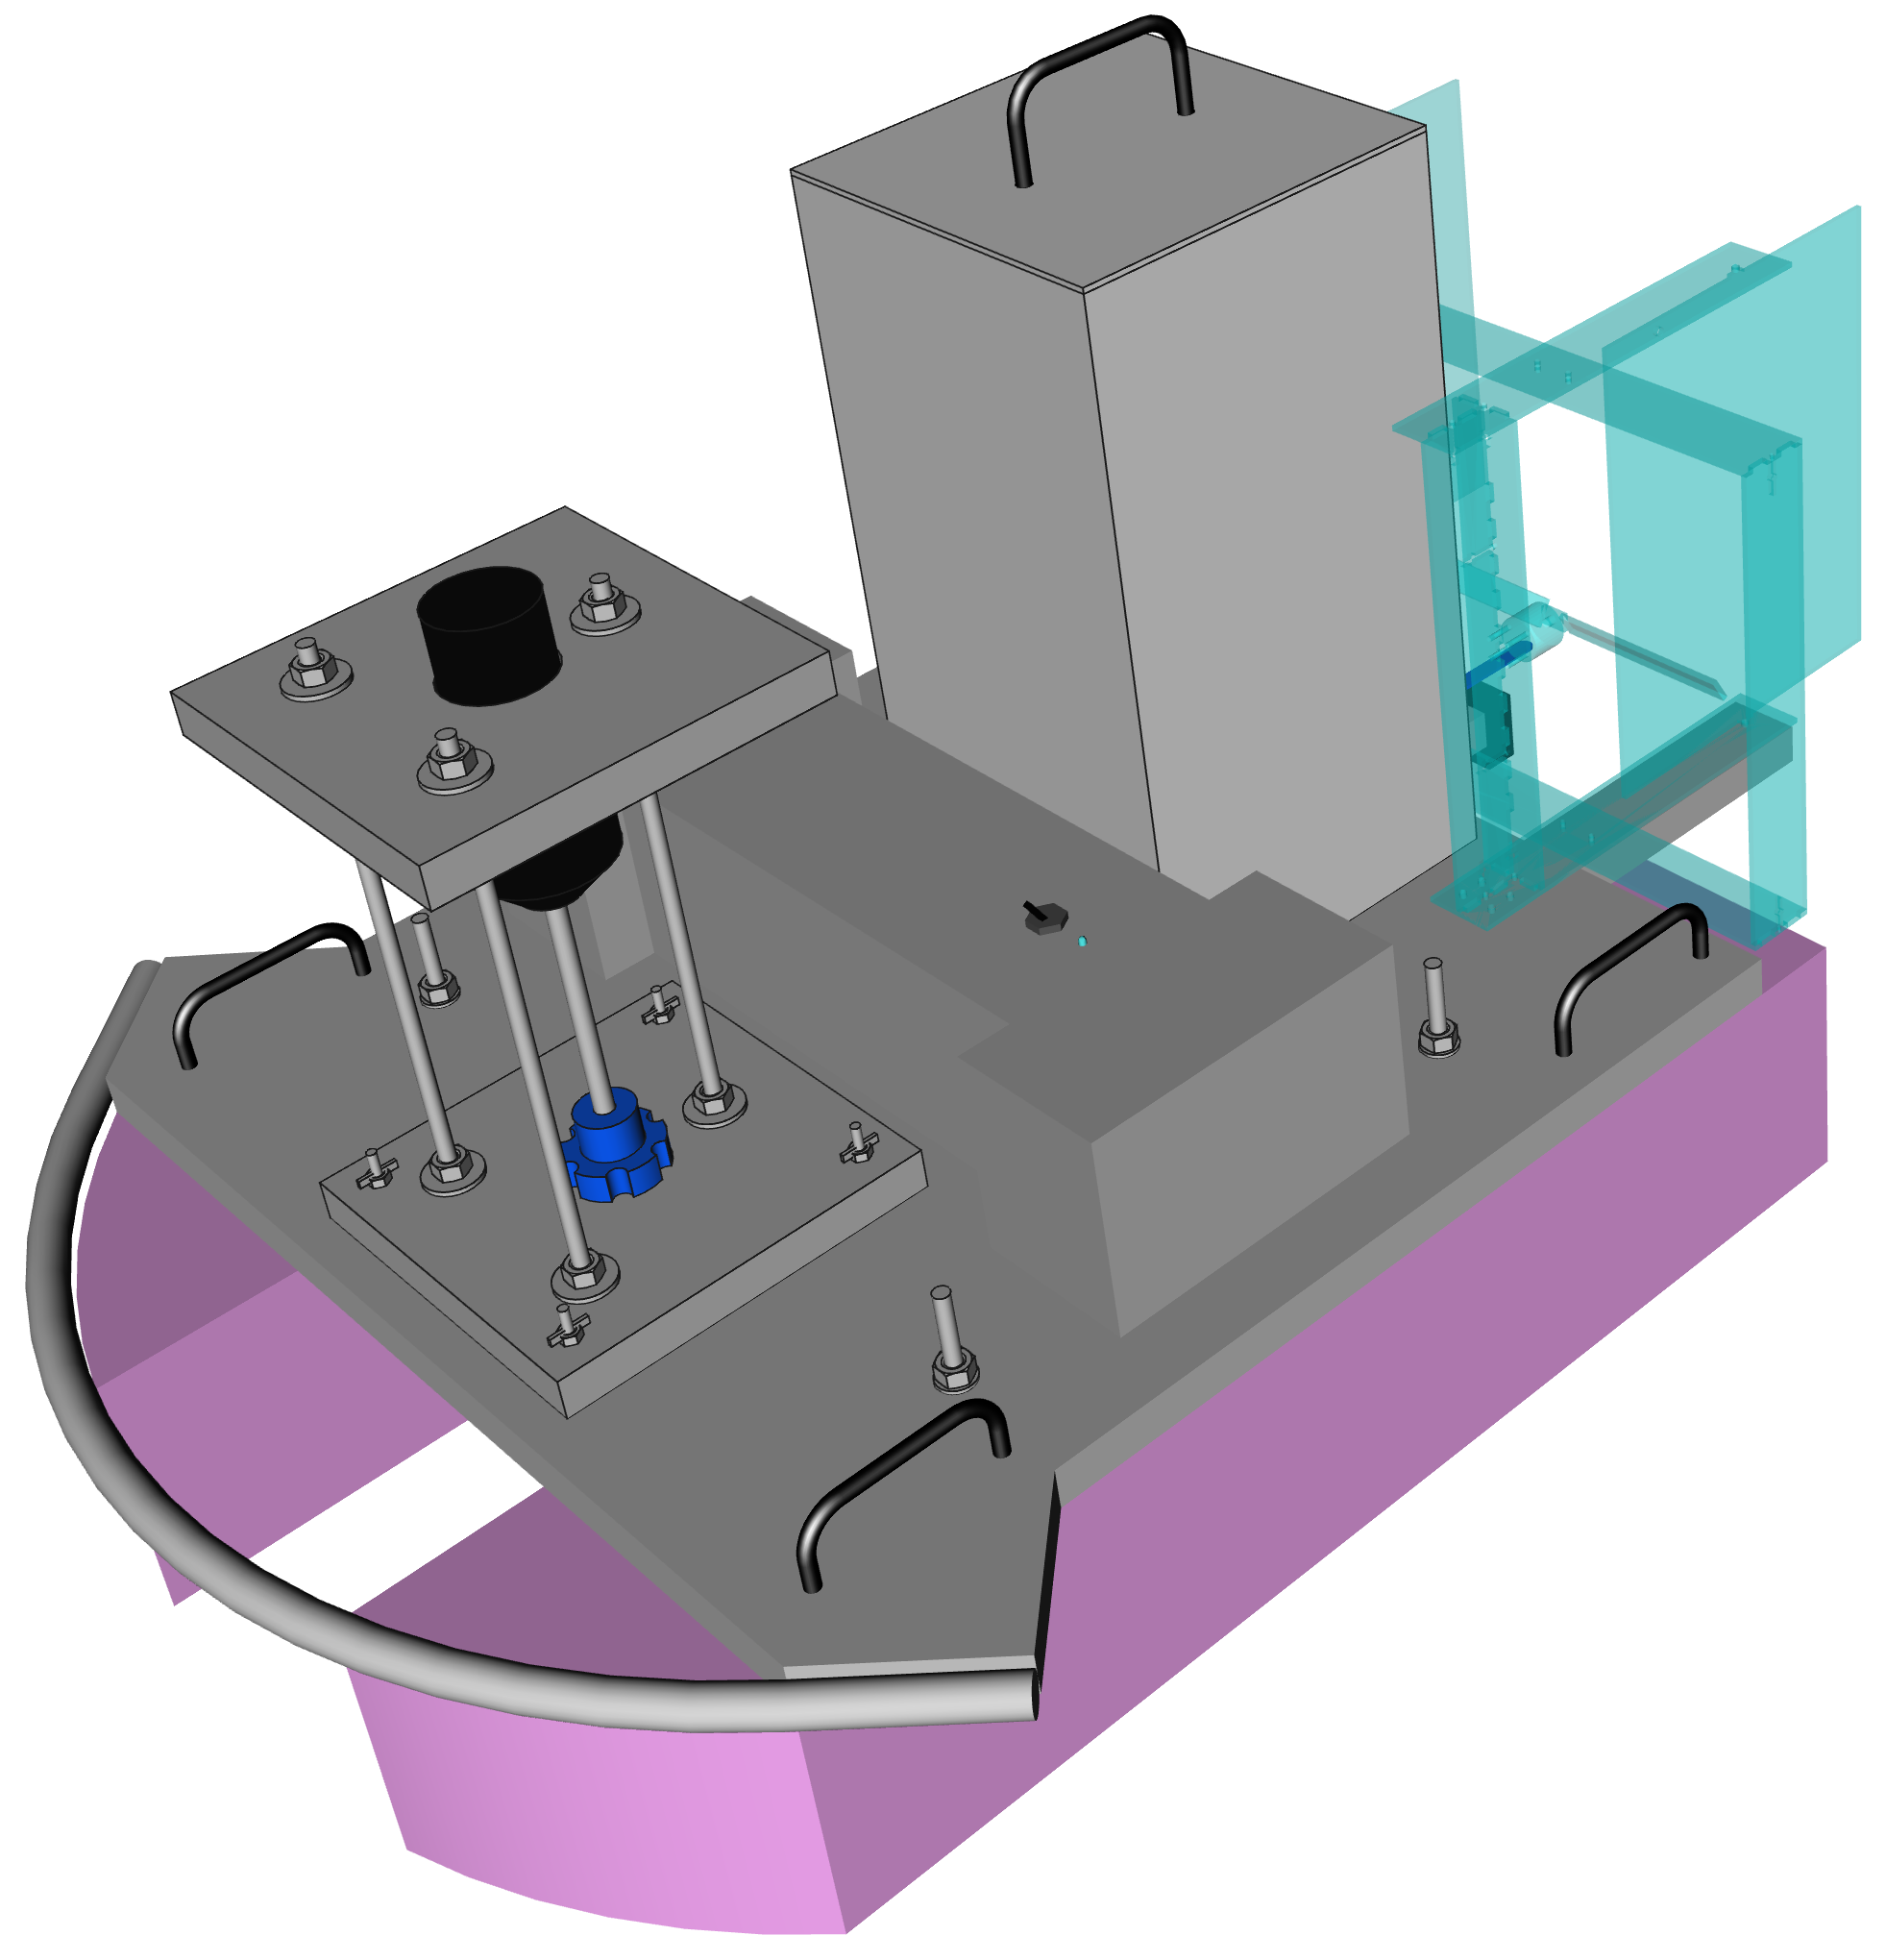
\includegraphics[width=27cm]{figures/front_box_off.png}}
        \end{figure}

      \end{block}

    \end{column}
    \begin{column}{\onecolwid}

      \begin{block}{Färdig prototyp}
        \begin{itemize}
        \item Billig att tillverka. Använder många färdiga komponenter.
        \item Till stor del återvinnigsbar.
        \item God manöverbarhet.
          \item Tillräcklig batterikapacitet för att förbruka reaktanterna innan batterierna är förbrukade.
        \end{itemize}

        \vskip 8cm
        \begin{figure}[H]
          \centering
          \hbox{\hspace{-3cm}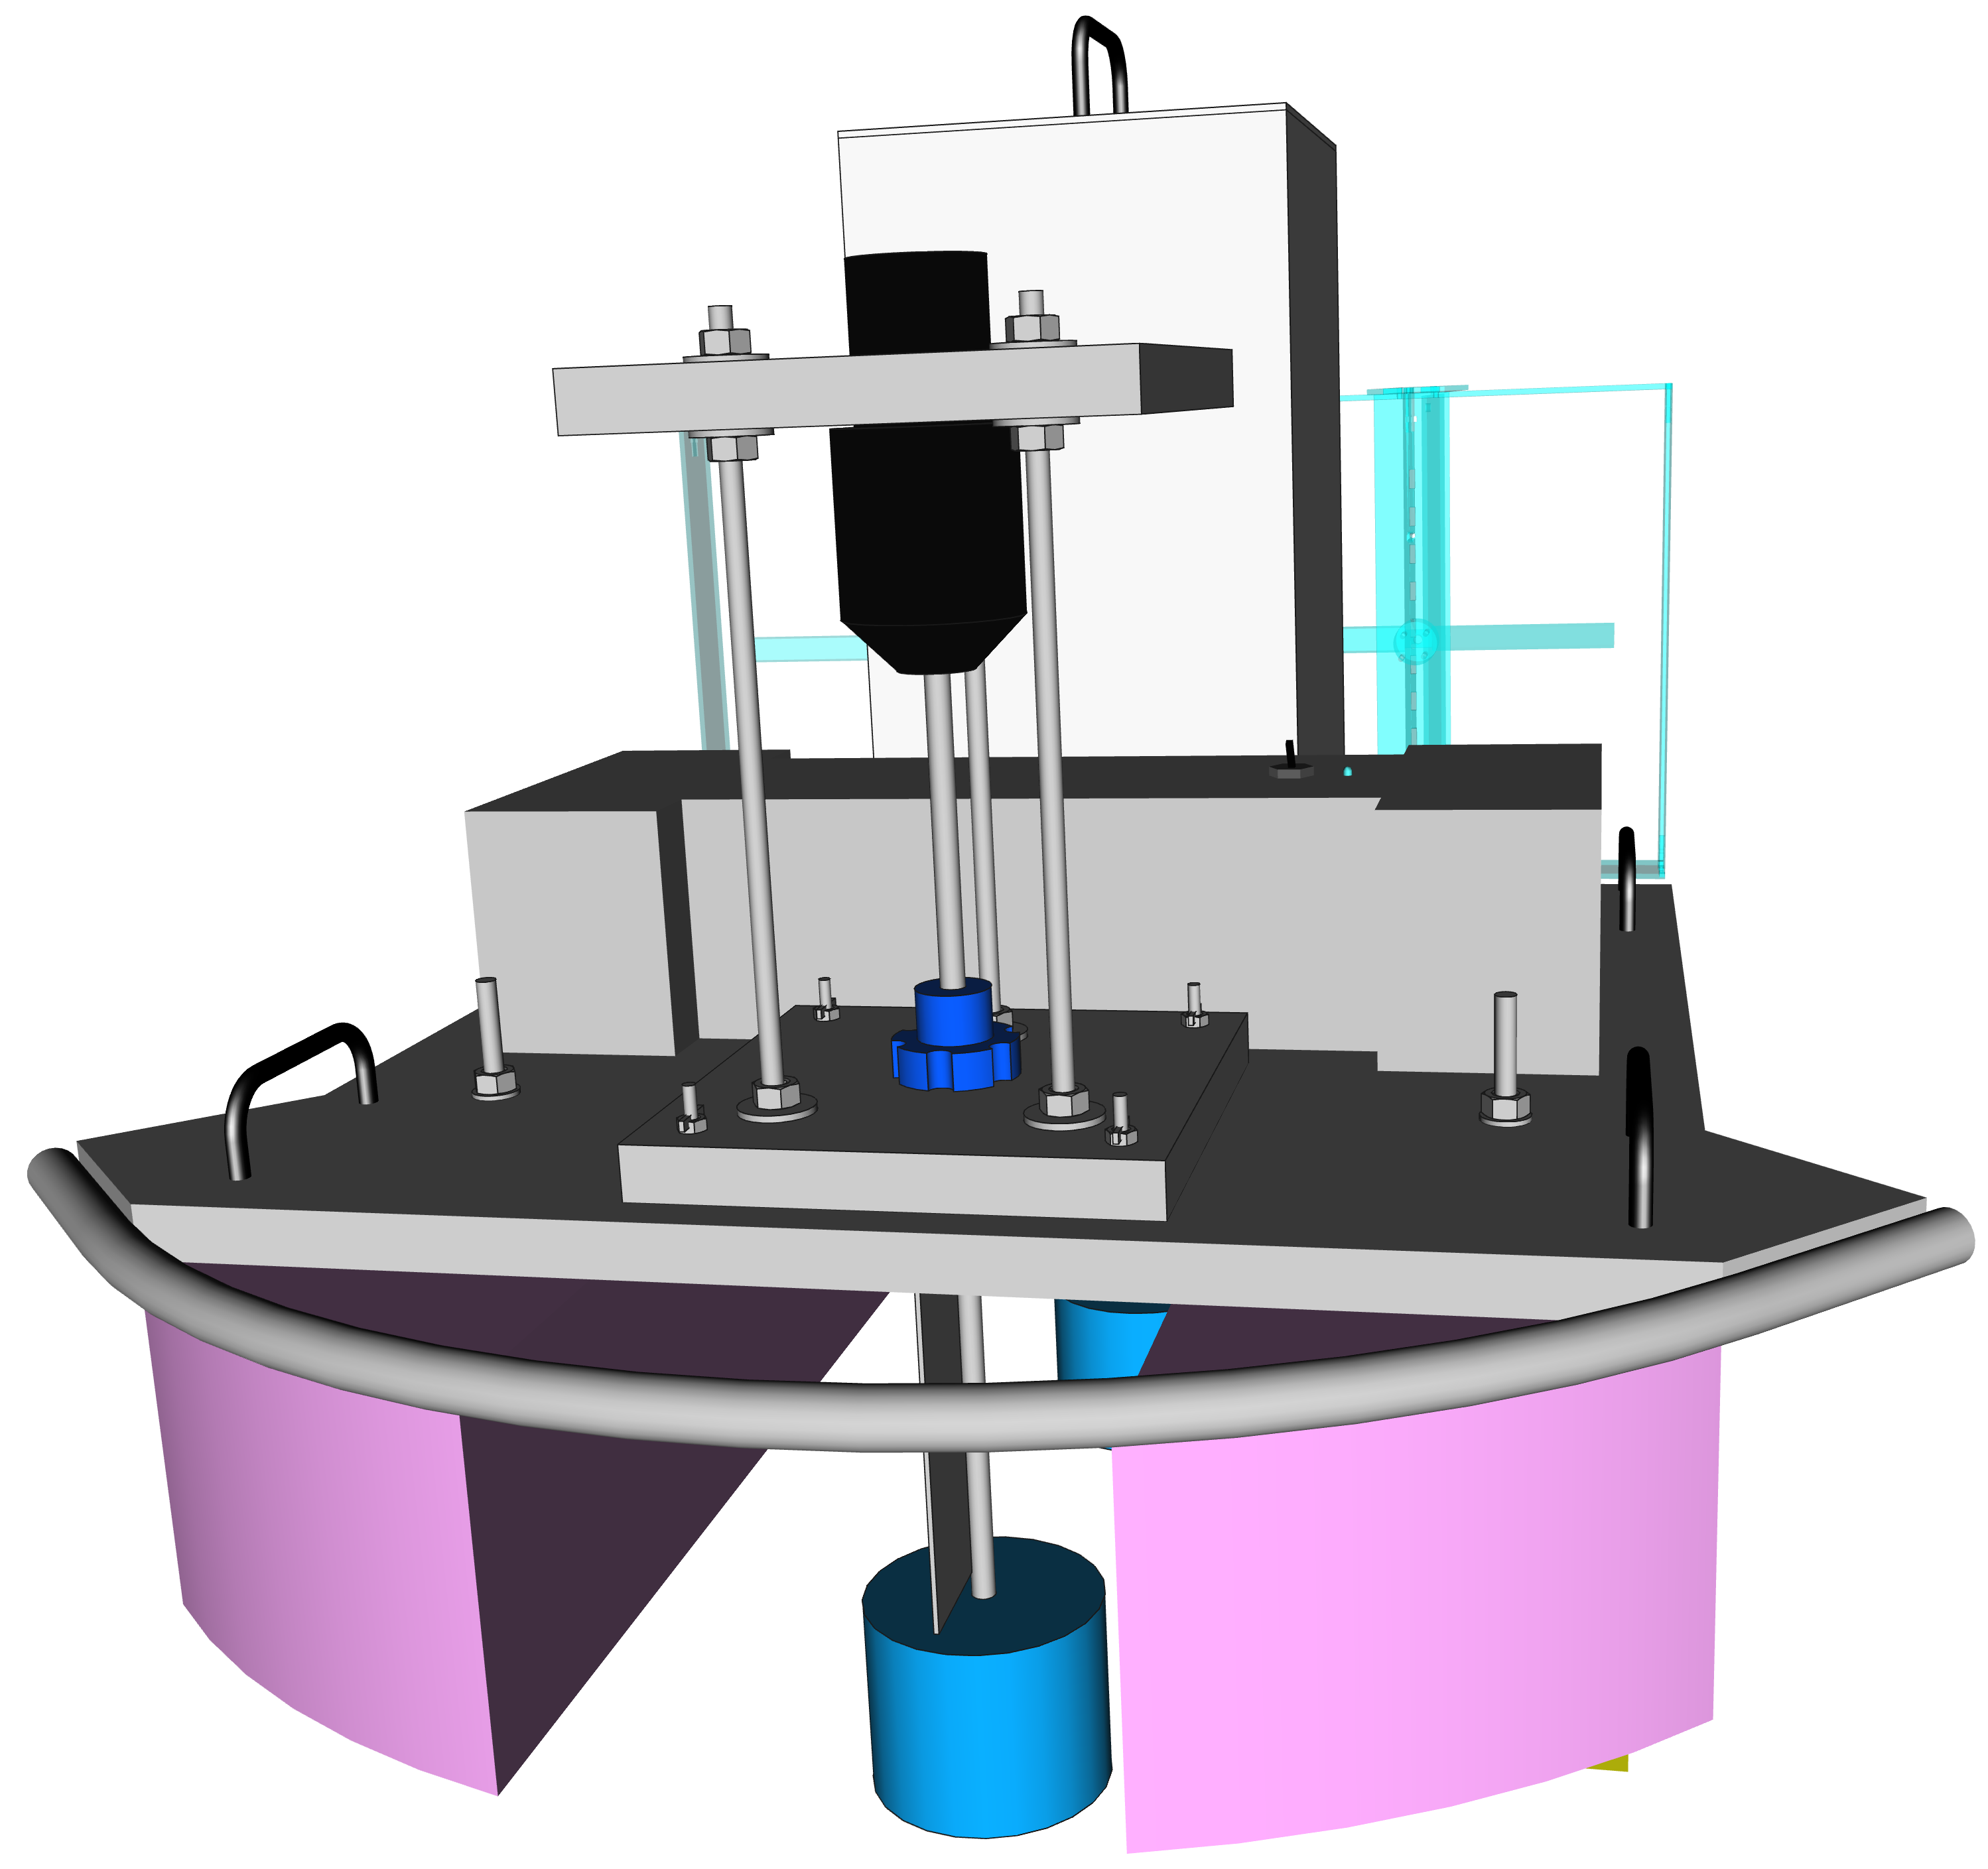
\includegraphics[width=25cm]{figures/front_rbr.png}}
        \end{figure}
      \end{block}

    \end{column}
    \begin{column}{\onecolwid}

      \begin{block}{Testresultat}
        \begin{itemize}
        \item Flotten kan rena 2~m$^3$ förorenat vatten på ungefär tio minuter.
        \item Bättre effekt än lokal stationär rening i samma vattenmassa.
        \end{itemize}

        \vskip 2cm
        \begin{figure}[H]
          \centering
          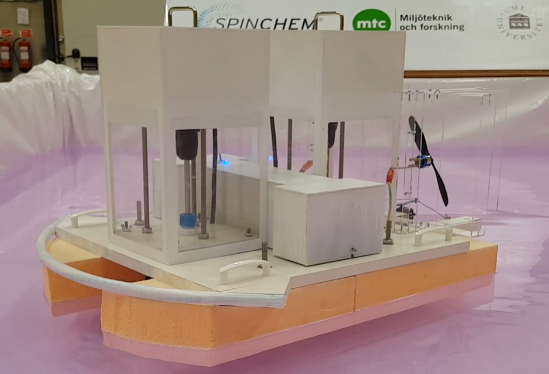
\includegraphics[width=\linewidth]{figures/flotte.png}
          \caption{Prototyp av robotflotten.}
        \end{figure}

        \vskip 2cm
        \begin{figure}[H]
          \centering
          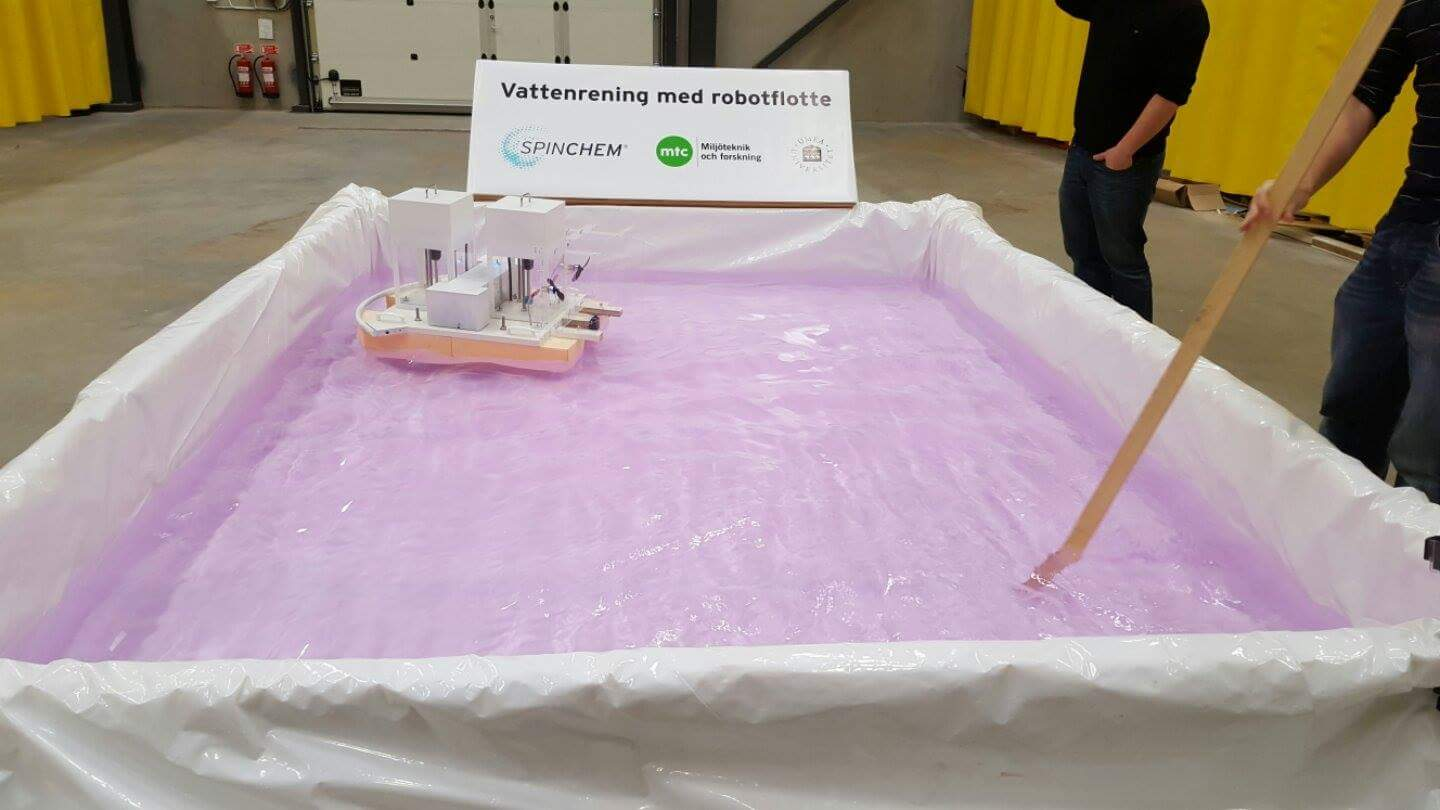
\includegraphics[width=\linewidth]{figures/pool.jpeg}
          \caption{Test i bassäng på Miljötekniskt Center i Umeå.}
        \end{figure}
      \end{block}

    \end{column}

  \end{columns} % End of all the columns in the poster

\end{frame} % End of the enclosing frame

\end{document}
